% Options for packages loaded elsewhere
\PassOptionsToPackage{unicode}{hyperref}
\PassOptionsToPackage{hyphens}{url}
%
\documentclass[
  english,
  man,floatsintext]{apa6}
\usepackage{amsmath,amssymb}
\usepackage{lmodern}
\usepackage{ifxetex,ifluatex}
\ifnum 0\ifxetex 1\fi\ifluatex 1\fi=0 % if pdftex
  \usepackage[T1]{fontenc}
  \usepackage[utf8]{inputenc}
  \usepackage{textcomp} % provide euro and other symbols
\else % if luatex or xetex
  \usepackage{unicode-math}
  \defaultfontfeatures{Scale=MatchLowercase}
  \defaultfontfeatures[\rmfamily]{Ligatures=TeX,Scale=1}
\fi
% Use upquote if available, for straight quotes in verbatim environments
\IfFileExists{upquote.sty}{\usepackage{upquote}}{}
\IfFileExists{microtype.sty}{% use microtype if available
  \usepackage[]{microtype}
  \UseMicrotypeSet[protrusion]{basicmath} % disable protrusion for tt fonts
}{}
\makeatletter
\@ifundefined{KOMAClassName}{% if non-KOMA class
  \IfFileExists{parskip.sty}{%
    \usepackage{parskip}
  }{% else
    \setlength{\parindent}{0pt}
    \setlength{\parskip}{6pt plus 2pt minus 1pt}}
}{% if KOMA class
  \KOMAoptions{parskip=half}}
\makeatother
\usepackage{xcolor}
\IfFileExists{xurl.sty}{\usepackage{xurl}}{} % add URL line breaks if available
\IfFileExists{bookmark.sty}{\usepackage{bookmark}}{\usepackage{hyperref}}
\hypersetup{
  pdftitle={Netflix case study: Genre vs decade},
  pdfauthor={Alan Kreher, Chantal van de Luijtgaarden, Dion Verschuren, Dylan van Wonderen, Suzanne Ekhart, \& Tawab Ghorbandi},
  pdflang={en-EN},
  pdfkeywords={keywords},
  hidelinks,
  pdfcreator={LaTeX via pandoc}}
\urlstyle{same} % disable monospaced font for URLs
\usepackage{graphicx}
\makeatletter
\def\maxwidth{\ifdim\Gin@nat@width>\linewidth\linewidth\else\Gin@nat@width\fi}
\def\maxheight{\ifdim\Gin@nat@height>\textheight\textheight\else\Gin@nat@height\fi}
\makeatother
% Scale images if necessary, so that they will not overflow the page
% margins by default, and it is still possible to overwrite the defaults
% using explicit options in \includegraphics[width, height, ...]{}
\setkeys{Gin}{width=\maxwidth,height=\maxheight,keepaspectratio}
% Set default figure placement to htbp
\makeatletter
\def\fps@figure{htbp}
\makeatother
\setlength{\emergencystretch}{3em} % prevent overfull lines
\providecommand{\tightlist}{%
  \setlength{\itemsep}{0pt}\setlength{\parskip}{0pt}}
\setcounter{secnumdepth}{-\maxdimen} % remove section numbering
% Make \paragraph and \subparagraph free-standing
\ifx\paragraph\undefined\else
  \let\oldparagraph\paragraph
  \renewcommand{\paragraph}[1]{\oldparagraph{#1}\mbox{}}
\fi
\ifx\subparagraph\undefined\else
  \let\oldsubparagraph\subparagraph
  \renewcommand{\subparagraph}[1]{\oldsubparagraph{#1}\mbox{}}
\fi
% Manuscript styling
\usepackage{upgreek}
\captionsetup{font=singlespacing,justification=justified}

% Table formatting
\usepackage{longtable}
\usepackage{lscape}
% \usepackage[counterclockwise]{rotating}   % Landscape page setup for large tables
\usepackage{multirow}		% Table styling
\usepackage{tabularx}		% Control Column width
\usepackage[flushleft]{threeparttable}	% Allows for three part tables with a specified notes section
\usepackage{threeparttablex}            % Lets threeparttable work with longtable

% Create new environments so endfloat can handle them
% \newenvironment{ltable}
%   {\begin{landscape}\centering\begin{threeparttable}}
%   {\end{threeparttable}\end{landscape}}
\newenvironment{lltable}{\begin{landscape}\centering\begin{ThreePartTable}}{\end{ThreePartTable}\end{landscape}}

% Enables adjusting longtable caption width to table width
% Solution found at http://golatex.de/longtable-mit-caption-so-breit-wie-die-tabelle-t15767.html
\makeatletter
\newcommand\LastLTentrywidth{1em}
\newlength\longtablewidth
\setlength{\longtablewidth}{1in}
\newcommand{\getlongtablewidth}{\begingroup \ifcsname LT@\roman{LT@tables}\endcsname \global\longtablewidth=0pt \renewcommand{\LT@entry}[2]{\global\advance\longtablewidth by ##2\relax\gdef\LastLTentrywidth{##2}}\@nameuse{LT@\roman{LT@tables}} \fi \endgroup}

% \setlength{\parindent}{0.5in}
% \setlength{\parskip}{0pt plus 0pt minus 0pt}

% \usepackage{etoolbox}
\makeatletter
\patchcmd{\HyOrg@maketitle}
  {\section{\normalfont\normalsize\abstractname}}
  {\section*{\normalfont\normalsize\abstractname}}
  {}{\typeout{Failed to patch abstract.}}
\patchcmd{\HyOrg@maketitle}
  {\section{\protect\normalfont{\@title}}}
  {\section*{\protect\normalfont{\@title}}}
  {}{\typeout{Failed to patch title.}}
\makeatother
\shorttitle{SNA4DS Research Project Report - Team 14}
\keywords{keywords\newline\indent Word count: X}
\usepackage{csquotes}
\ifxetex
  % Load polyglossia as late as possible: uses bidi with RTL langages (e.g. Hebrew, Arabic)
  \usepackage{polyglossia}
  \setmainlanguage[]{english}
\else
  \usepackage[main=english]{babel}
% get rid of language-specific shorthands (see #6817):
\let\LanguageShortHands\languageshorthands
\def\languageshorthands#1{}
\fi
\ifluatex
  \usepackage{selnolig}  % disable illegal ligatures
\fi
\newlength{\cslhangindent}
\setlength{\cslhangindent}{1.5em}
\newlength{\csllabelwidth}
\setlength{\csllabelwidth}{3em}
\newenvironment{CSLReferences}[2] % #1 hanging-ident, #2 entry spacing
 {% don't indent paragraphs
  \setlength{\parindent}{0pt}
  % turn on hanging indent if param 1 is 1
  \ifodd #1 \everypar{\setlength{\hangindent}{\cslhangindent}}\ignorespaces\fi
  % set entry spacing
  \ifnum #2 > 0
  \setlength{\parskip}{#2\baselineskip}
  \fi
 }%
 {}
\usepackage{calc}
\newcommand{\CSLBlock}[1]{#1\hfill\break}
\newcommand{\CSLLeftMargin}[1]{\parbox[t]{\csllabelwidth}{#1}}
\newcommand{\CSLRightInline}[1]{\parbox[t]{\linewidth - \csllabelwidth}{#1}\break}
\newcommand{\CSLIndent}[1]{\hspace{\cslhangindent}#1}

\title{Netflix case study: Genre vs decade}
\author{Alan Kreher\textsuperscript{}, Chantal van de Luijtgaarden\textsuperscript{}, Dion Verschuren\textsuperscript{}, Dylan van Wonderen\textsuperscript{}, Suzanne Ekhart\textsuperscript{}, \& Tawab Ghorbandi\textsuperscript{}}
\date{}


\affiliation{\vspace{0.5cm}\textsuperscript{1} Jheronimus Academy of Data Science\\\textsuperscript{2} Eindhoven University of Technology\\\textsuperscript{3} Tilburg University}

\begin{document}
\maketitle

{
\setcounter{tocdepth}{3}
\tableofcontents
}
\hypertarget{citations-in-papaja-detele-appropriately-later}{%
\section{Citations in papaja, detele appropriately later}\label{citations-in-papaja-detele-appropriately-later}}

Add the bibtex entry in the .bib file. You can find the entries in Google scholar,
but double check since it is not always correct.

Call the citations in the text:

Citation within parentheses (Aust \& Barth, 2020)

Multiple citations (Aust \& Barth, 2020; R Core Team, 2021)

In-text citations Aust and Barth (2020)

Year only (2021)

Only if your citation appears in the text it will also show up in the Reference
list. Don't manually modify the Reference list.

\hypertarget{executive-summary}{%
\subsection{Executive Summary}\label{executive-summary}}

(150 words) -- 0.3 POINTS
Summarize the report. Write this as the very last thing.

What is the main topic you are addressing?

what are your research questions and hypotheses?

what are your results and the main conclusion?

\hypertarget{introduction}{%
\subsection{Introduction}\label{introduction}}

\hypertarget{main-topic}{%
\subsubsection{Main topic}\label{main-topic}}

In this paper, we are going to study the presence of social networks within a movie streaming platform. We're focusing on the structure of links among a group of social players, which consist of users watching and rating movies on Netflix.\\
Users of Netflix's movie recommendation algorithms are frequently given specific questions about their interests for certain items (which they provide by liking or disliking them, for example). These choices are then immediately integrated into the underlying learning system for future suggestions. If a recommender system starts promoting unwanted products after incorporating new preferences, the user may try to steer the system in the future by correcting it or supplying alternate preference information.

\hypertarget{importance}{%
\subsubsection{Importance}\label{importance}}

It is important to study the presence of these socials networks because this could potentially improve the recommender engine that this currently in place. For example, if you know that a user is likely to like a movie that other users with the same ``liking profile'' also like, you can recommend that movie to the user. When these connections are studied thoroughly, you could have a high probability that the recommendation is successful. This could have a large impact on a movie streaming platform.

\hypertarget{existing-studies}{%
\subsubsection{Existing studies}\label{existing-studies}}

In this paper, we will be looking into the Netflix Price Dataset. In 2006 Netflix decided to start a competition with a grand prize of 1 million US dollars. The goal of the competition was to create a collaborative filtering algorithm to predict user ratings for films, based on previous ratings without any other information about the users or films. In order to win you had to at least improve on Netflix's own algorithm by 10\%.
During the competition a lot of literature has emerged about the dataset and the competition. (Bell \& Koren, 2007; Narayanan \& Shmatikov, 2006; Takács, Pilászy, Németh, \& Tikk, 2008)

However, no papers or any other literature can be found on network analysis on this dataset. We like to fill this gap in the literature by analysing the network and network structure that arises from the subset of the data that we will use.
(Guillory \& Bilmes, 2011) developed an active movie recommendation system for Netflix. They found that a recommender system should not constantly ask questions to a user, because those reduces the user's mental image of how the recommendation system learns, prompting some participants to ``lose track of what they were teaching.'' According to Amershi, Cakmak, Knox, and Kulesza (2014), this was because users are not always eager to act as simple oracles (repeatedly telling the recommendation system whether they like something or not). This is interesting to take into account for our research, because this would mean that a social network within a movie recommendation system can never be fully exposed.

\hypertarget{research-questions-and-hypotheses}{%
\subsubsection{Research Questions and hypotheses}\label{research-questions-and-hypotheses}}

In this dataset, we can easily see connections between users and movies, but not between just the users or just the movies. At least not, when we do not include one or the other. That is why we have defined the following research questions:

\begin{itemize}
\tightlist
\item
  RQ1: What are the effects of the genre on the likelihood of having both movies watched by the same user?
\item
  RQ2: How much does liking the same movies influence disliking the same movies, and vice versa? (In a network of frequent reviewers)
\end{itemize}

In order to be able to answer these research questions, we have made set up the following hypothesis accordingly:

\begin{itemize}
\tightlist
\item
  Research Question 1:

  \begin{itemize}
  \tightlist
  \item
    Comparable movies, in terms of either genre and/or year, are more often watched by the same user than uncomparable movies.\\
  \item
    Movies of genre horror are generally rated higher than other movie genres.
  \end{itemize}
\item
  Research Question 2:

  \begin{itemize}
  \tightlist
  \item
    Users that like the same movies to a certain degree, are likely to dislike the same movies to that same degree
  \item
    Users that dislike the same movies to a certain degree, are likely to like the same movies to that same degree
  \end{itemize}
\end{itemize}

\hypertarget{methodology}{%
\subsection{Methodology}\label{methodology}}

\hypertarget{dataset}{%
\subsubsection{Dataset}\label{dataset}}

The primary dataset that is being used during this study is provided by Netflix (REF: KAGGLE) .
Netflix shared this data for the Netflix Prize competition where people could use the data to improve their recomender system for movies.
The data includes ratings for 17770 movies from 480189 users.
In total, it contains around 24 million ratings on a scale from one to five and the date of the rating.
For the movies, the dataset only contains the title of the movie and the year it was released.
This was too little information about the movies for our project.
Therefore, we decided to look for an additional data source to enrich the dataset.
We used Amazon Prime movie genres to add genres to the dataset for further analysis.

The large size of the dataset made it difficult to work with and made running analysis models infeasable.
Therefore, we decided to only use a selection of the ratings. The dataset has ratings from October 1998 to December 2005.
For this analysis, only the data from December 2001, Januari 2002, and februari 2002 are considered.
We chose this winter because this is the first time where users started to rate a good amount of movies while the number of ratings still did not completely explode yet.

To answer our two research questions we had to transform our data further in two different ways.
For the first research question, the network is defined as movies for the nodes and the movies have an edge between them if there is an user that likes both movies.
Liking a movie is defined as a user giving a 4 or 5 rating for a movie.
Of course, modelling the network this way means that movies that are highly rated are always connect.
Therefore, the network only included movies that have between 20 and 50 ratings.
That means that our analysis only concerns niche movies with a small number of ratings.
Moreover, there is a lower threshold too to make sure that we only include movies that have at least a few connections.
All in all, the network is just under 500 nodes and the attributes for the nodes are the year of release of the movie and the main movie genre that comes from Amazon Prime.

\hypertarget{descriptives}{%
\paragraph{Descriptives}\label{descriptives}}

Looking at the average Rating of the users in the data, the average rating they gave was about a \(3,36\).

\begin{table}
\centering
\begin{tabular}{l|r|r|r|r|r}
\hline
  & mean & sd & min & max & n\\
\hline
Rating & 3.362346 & 1.114827 & 1 & 5 & 864610\\
\hline
\end{tabular}
\end{table}

Looking at the histogram of the amound of ratings given on a certain date we can see that a peak in ratings exists always in the middle of the week (around wednesday/thursday). Looking at the distribution of the ratings over time we don't see great differences. Over time, people give consistent ratings.

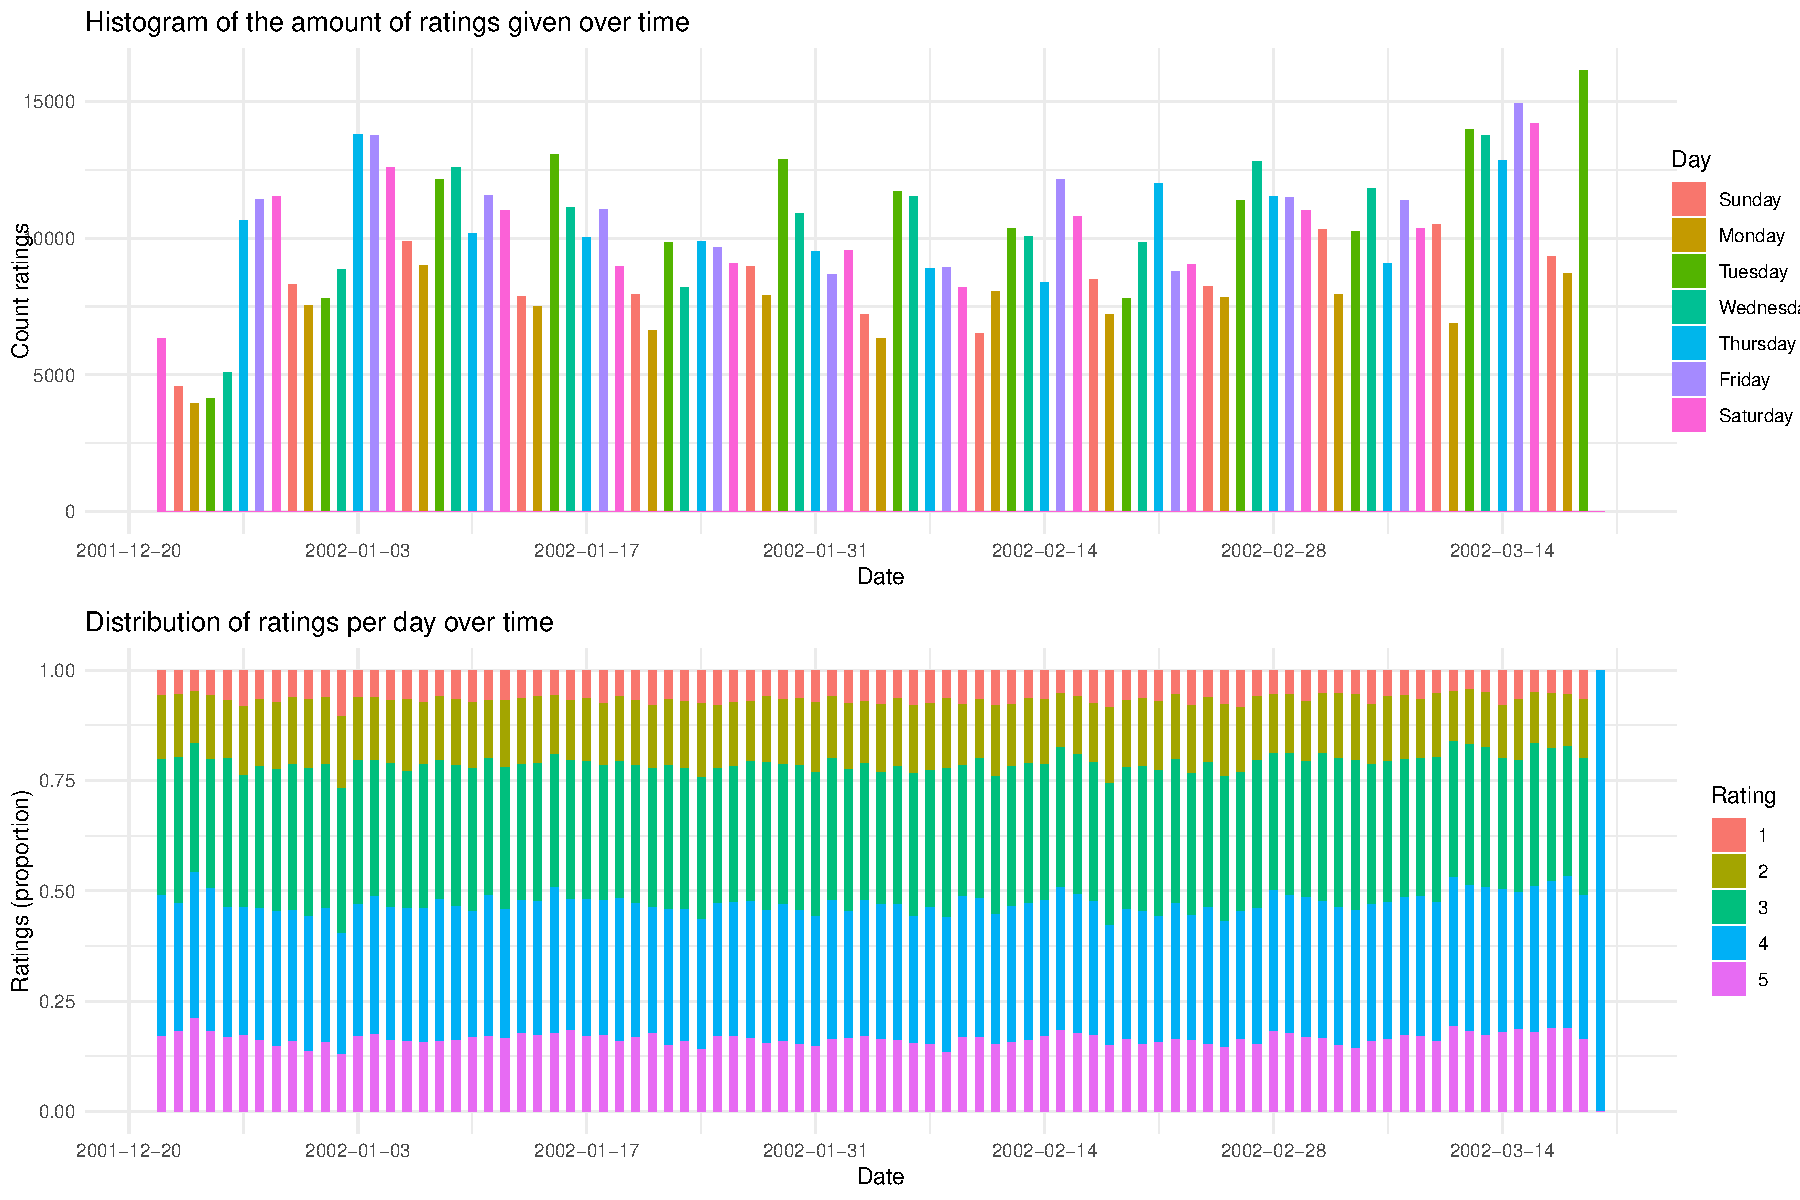
\includegraphics{SNA4DSprojectReport_files/figure-latex/unnamed-chunk-5-1.pdf}

The genres in the data were determined using Amazone Prime. The first genre that Amazone Prime displayed is taken as the genre of the movie. As the genres that were displayed in Amazone Prime were not on alfabethic order, we assume that the first genre given is the main genre. 20 genres were found in the Netflix dataset. Most of the movies had \emph{comedy} or \emph{drama} as genre.

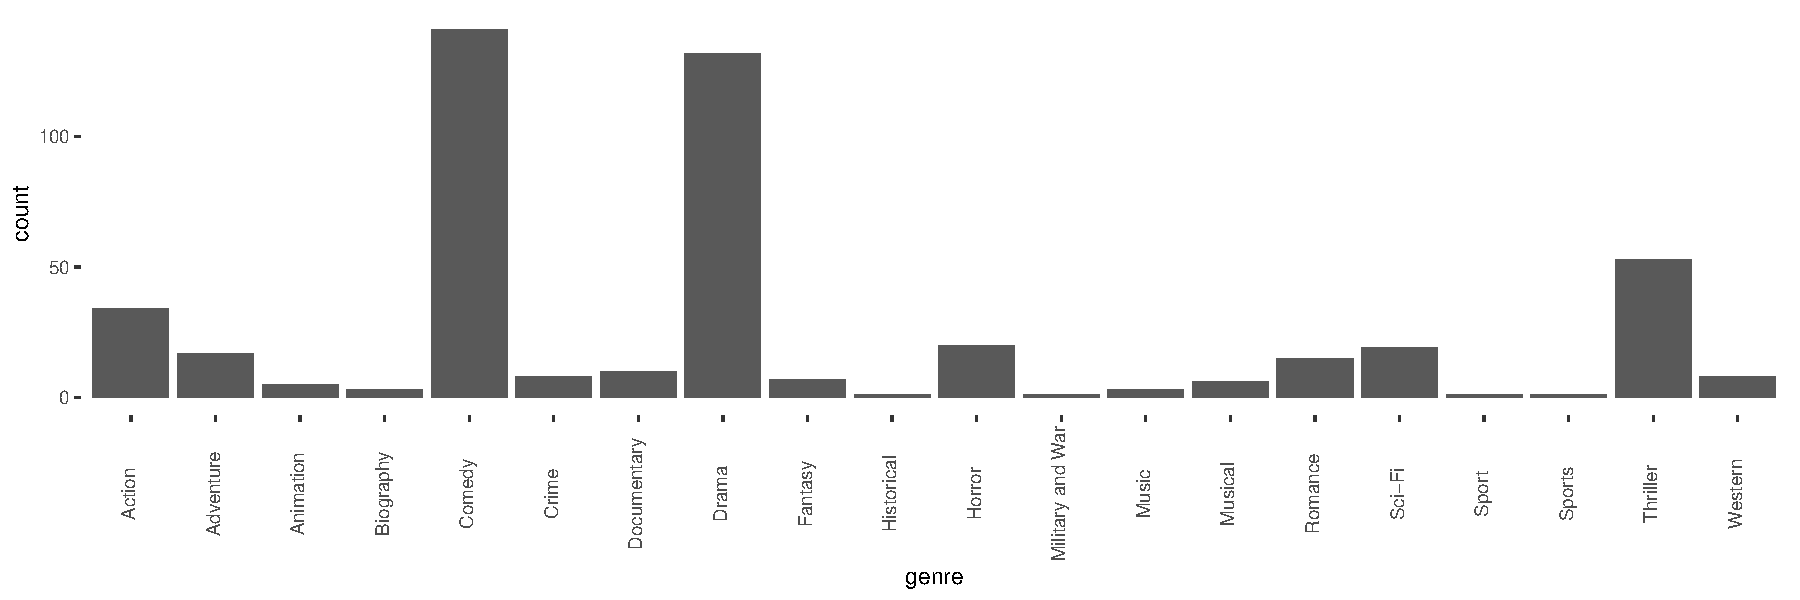
\includegraphics{SNA4DSprojectReport_files/figure-latex/unnamed-chunk-6-1.pdf}

\hypertarget{data-analysis-research-rationale}{%
\subsubsection{Data analysis (Research Rationale)}\label{data-analysis-research-rationale}}

\hypertarget{ergm}{%
\paragraph{ERGM}\label{ergm}}

Many metrics like density and centrality are used to describe the structural characteristics of an observed network. These metrics, on the other hand, describe the observed network, which is just one of many possible alternative networks. The structural characteristics of this group of alternative networks may or may not be similar. A statistical model must consider the set of all possible alternative networks weighted in their similarity to an observed network to credit a statistical inference about the processes that influence the formation of network structures.

Network data, on the other hand, violates the independence and identical distribution assumptions of statistical models like linear regression because they are inherently relational. Alternative statistical models must reflect the uncertainty associated with a given observation and allow inference about the relative frequency of theoretically important network substructures. Exponential Random Graph Models (ERGM) help with this.

Using ERGMs is a powerful technique for conducting statistical inference on network data. ERGMs are a good choice as a network modelling framework for cases where the outcome of interest is in the presence or absence of edges.

\hypertarget{qap}{%
\paragraph{QAP}\label{qap}}

In general, QAP is very interesting, when you have two or more networks and wants to compare those. In addition, we also choose QAP regression, since we thought it would be interesting to use this model, based on its permutation of actually observed graphs and therefore staying closer to the nature of our networks.

There are three different QAP models from which one had to be chosen for our data and research question. The first is the simple QAP test where you measure the association between two networks. Furthermore, there is a QAP linear model, which can be used on a valued dependent network and one or more explanatory networks. Finally, there is the QAP logistic model, which differs from the linear model, in terms of a binary-valued dependent network.

Our weights in our network are not binary so the logistic model is not an option for us. Even though, we only have two networks we decided to go for the linear model since we would like to see if we could ``explain'' the first network with the second and vice versa.

As QAP is the only method (to our knowledge) that is able to compare two networks to each other, there aren't any other methods available to address the second research question.

\hypertarget{results}{%
\subsection{Results}\label{results}}

\hypertarget{qap-model}{%
\subsubsection{QAP Model}\label{qap-model}}

\hypertarget{constructing-data-and-the-model}{%
\paragraph{Constructing data and the model}\label{constructing-data-and-the-model}}

During preprocessing of the data, an interesting artifact was encountered; When users were removed from the dataset that either liked or disliked a movie, it was clearly shown that it occurred much more often that user gave a 4/5 star rating to a movie than a 1/2 star rating. This is interesting to keep in mind, as this might pose a potential bias in the dataset.

To give a weight to the edges in terms of importance, we calculate the weight according to a formula:

\[weight = max((\frac{no. of mutual liked movies}{
no. of liked movies})*100) \]

\hypertarget{results-1}{%
\paragraph{Results}\label{results-1}}

We have generated results for different (filtered) versions of the dataset. The results are explained and shown below.

\hypertarget{more-than-120-reviews}{%
\subparagraph{More than 120 reviews}\label{more-than-120-reviews}}

In order to get a feeling of the QAP regression model, and to get initial results in a reasonable amount of time, we first did the analysis on users who had 120 reviews in total(like and dislike) or more. The results are shown in the figure below.

\begin{figure}
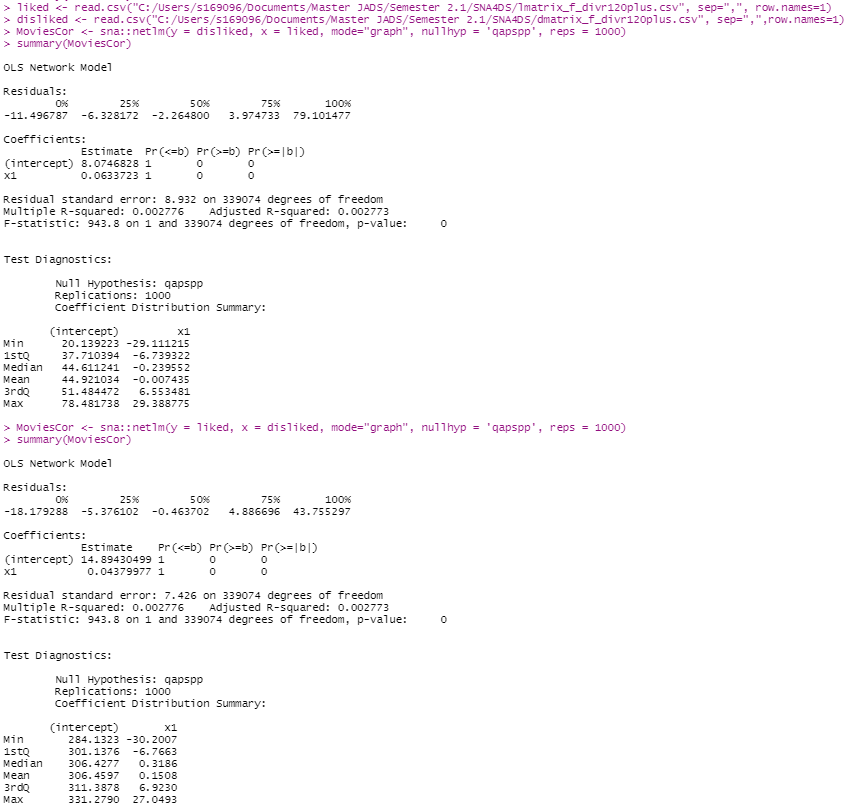
\includegraphics[width=2.85in]{results120plus} \caption{ }\label{fig:unnamed-chunk-7}
\end{figure}

As can be seen from the figure, the QAP regression model explains only 6\% of the variation in the like/dislike interaction network for movies when looking at liked movie ratings. When looking at disliked movie ratings, it becomes even less: 4\%.

\hypertarget{more-than-100-reviews}{%
\subparagraph{More than 100 reviews}\label{more-than-100-reviews}}

Next, we decreased the filter threshold for the number of ratings that users have given in the dataset. This increased the amount of datapoints in the dataset. So, we had a dataset with users who had 100 reviews in total (like and dislike) or more, and ran the analysis. The results are shown in the figure below.

\begin{figure}
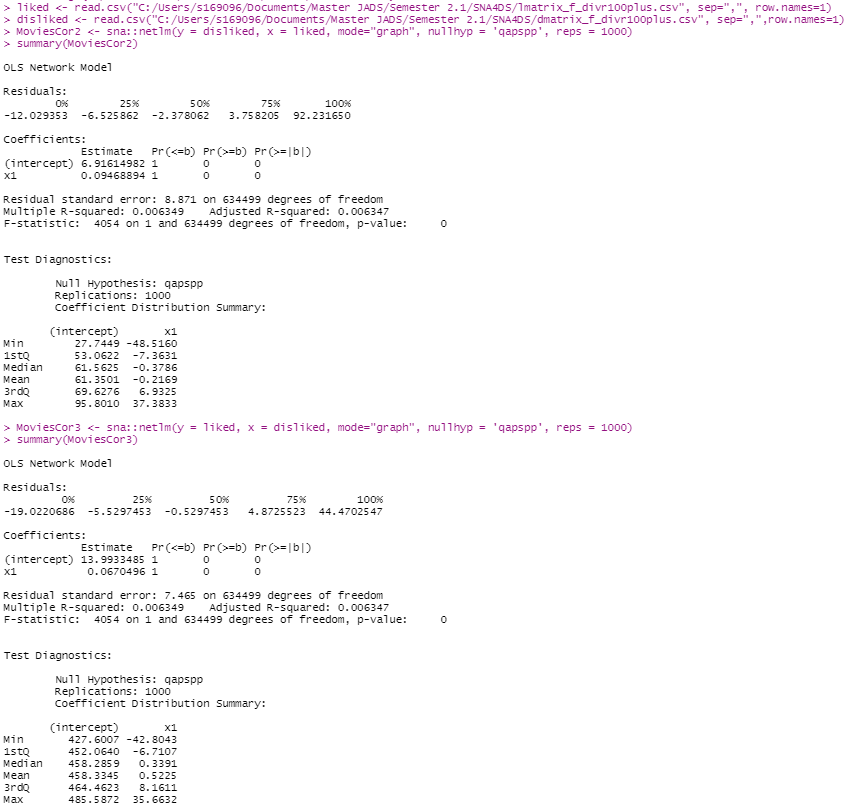
\includegraphics[width=2.89in]{results100plus} \caption{ }\label{fig:unnamed-chunk-8}
\end{figure}

As can be seen from the figure, the QAP regression model explains only 9\% of the variation in the like/dislike interaction network for movies when looking at liked movie ratings. When looking at disliked movie ratings, it becomes even less: 6\%.

\hypertarget{more-than-80-reviews}{%
\subparagraph{More than 80 reviews}\label{more-than-80-reviews}}

Because of the improved results in the last section, we decreased the filter threshold for the number of ratings that users have given in the dataset even more. This again increased the amount of datapoints in the dataset, and we did the analysis on users who had 80 reviews in total (like and dislike) or more. The results are shown in the figure below.

\begin{figure}
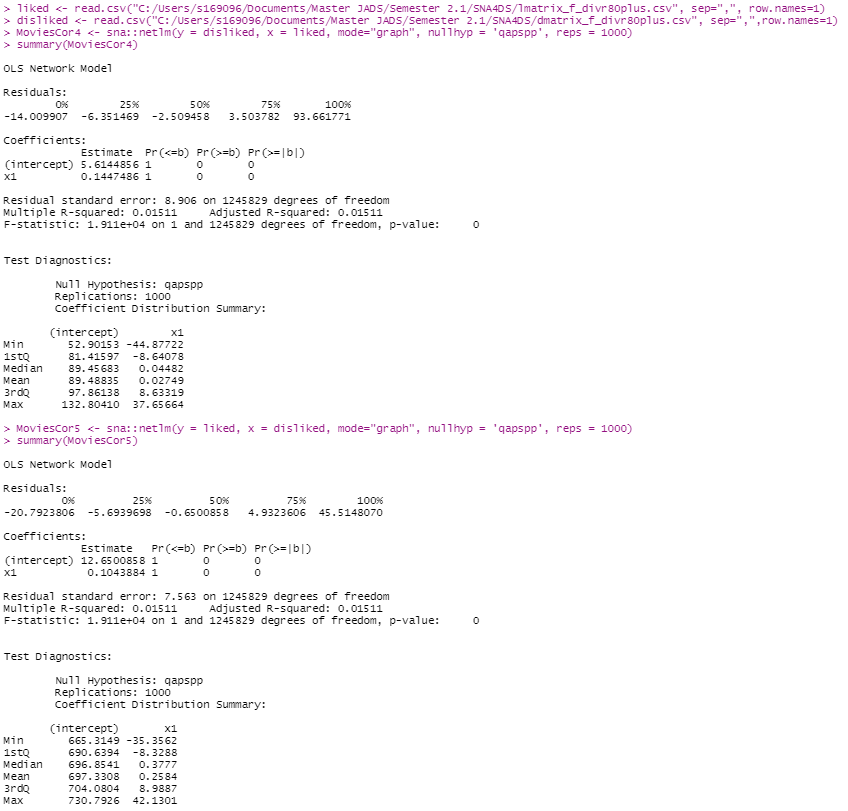
\includegraphics[width=2.83in]{results80plus} \caption{ }\label{fig:unnamed-chunk-9}
\end{figure}

As can be seen from the figure, the QAP regression model explains 14\% of the variation in the like/dislike interaction network for movies when looking at liked movie ratings. When looking at disliked movie ratings, it again becomes a bit less: 10,4\%.

\hypertarget{more-than-60-reviews}{%
\subparagraph{More than 60 reviews}\label{more-than-60-reviews}}

For the last time, we decreased the filter threshold for the number of ratings that users have given in the dataset. This also increased the amount of datapoints in the dataset, and we ran the analysis on users who had 80 reviews in total (like and dislike) or more. The results are shown in the figure below.

\begin{figure}
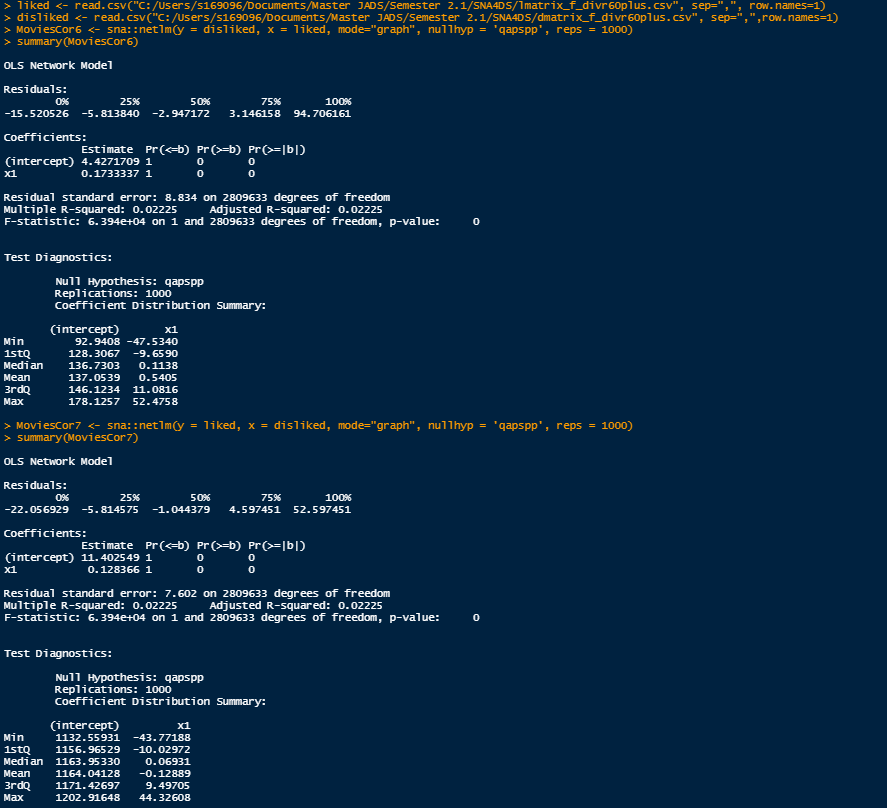
\includegraphics[width=2.95in]{results60plus} \caption{ }\label{fig:unnamed-chunk-10}
\end{figure}

As can be seen from the figure, the QAP regression model explains 17\% of the variation in the like/dislike interaction network for movies when looking at liked movie ratings. When looking at disliked movie ratings, the model can explain 13\% of the variation. Th finally gave us the feeling that we are building somewhat meaningful models.

We even wanted to go a step further and decrease the filter threshold for the number of ratings that users have given to 40. But this would yield a dataset that was too large to analyse, as it costs 25+ hours to run an analysis on it.

\hypertarget{findings-in-relation-to-hypothesis}{%
\paragraph{Findings in relation to hypothesis}\label{findings-in-relation-to-hypothesis}}

When relating our findings to our aforementioned hypothesis, we see that it is possible to build models that somewhat can explain the variance in the network in a significant way. However, we can clearly see that more data is not always giving better explanations.

Also, it very interesting to see that liking movies says more about which movies you might dislike, than vice versa. An explanation for this might be that we saw in the data that there were more positive ratings than negative ratings, which could explain that disliking defines a more specific taste that is better detectable.

\hypertarget{ergm-1}{%
\subsubsection{ERGM}\label{ergm-1}}

(about 1000) -- 2.5 POINTS

\begin{itemize}
\item
  Present your results appropriately (plots, tables\ldots) and discuss your findings
  in plain English
\item
  Discuss the meaning of your findings in relation to your hypothesis. (half of
  the points evaluated in this other part)
\end{itemize}

Option 1:

\begin{tabular}{l|l}
\hline
 & Model 1\\
\hline
(Intercept) & 5.03 ***\\
\hline
 & (0.22)\\
\hline
groupTrt & -0.37\\
\hline
 & (0.31)\\
\hline
R\textasciicircum{}2 & 0.07\\
\hline
Adj. R\textasciicircum{}2 & 0.02\\
\hline
Num. obs. & 20\\
\hline
\end{tabular}

Option 2

\begin{tabular}{l|l|l}
\hline
 & Model 1 & Model 2\\
\hline
(Intercept) & 5.03 *** & \\
\hline
 & (0.22) & \\
\hline
groupTrt & -0.37 & 4.66 ***\\
\hline
 & (0.31) & (0.22)\\
\hline
groupCtl &  & 5.03 ***\\
\hline
 &  & (0.22)\\
\hline
R\textasciicircum{}2 & 0.07 & 0.98\\
\hline
Adj. R\textasciicircum{}2 & 0.02 & 0.98\\
\hline
Num. obs. & 20 & 20\\
\hline
\end{tabular}

Option 3

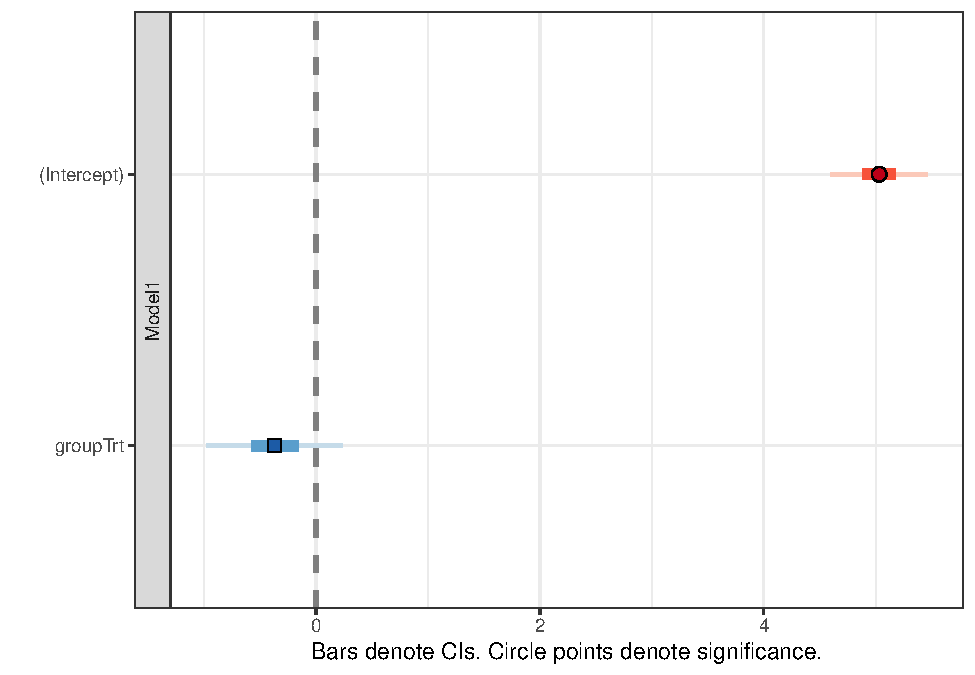
\includegraphics{SNA4DSprojectReport_files/figure-latex/model 3-1.pdf}

Option 4

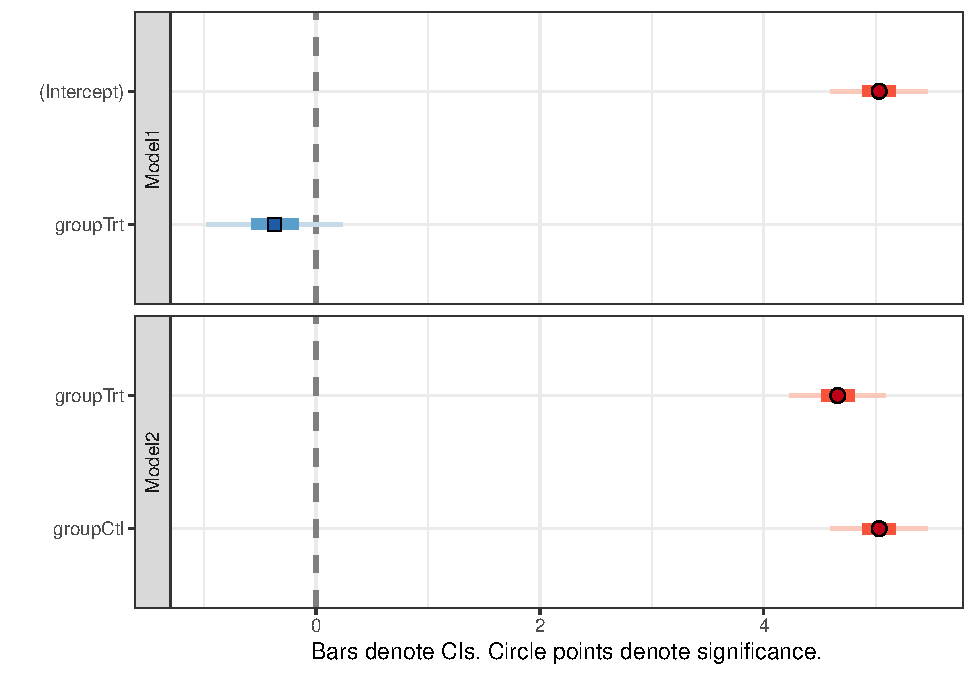
\includegraphics{SNA4DSprojectReport_files/figure-latex/model 4-1.pdf}

\hypertarget{conclusion}{%
\subsection{Conclusion}\label{conclusion}}

(about 350 words) -- 0.7 POINTS
What were your topic and research questions again? (1 sentence)

What did you learn from the two analysis you run? *** most important point to
address 0.5 POINTS here

Who benefits from your findings?

What does remain an open problem?

\hypertarget{discussion}{%
\subsubsection{Discussion}\label{discussion}}

What remains an open problem, is that we assume that a frequent reviewer gives a rating to a movie after watching it. However, we don't have information on (re-)viewers that watch a movie but don't give a rating afterwards. This is difficult to overcome as we simply don't have data available on this matter.

\textbf{\emph{Can you give suggestions for future work in this area?}}
For future research it could be beneficial to dive more into the literature and find out more about what is already known in order to give a stronger reasoning behind the explanatory variables used in the analysis. Also, it would be interesting to look into more recent data as streaming services are widely used nowadays and the variation of users is maybe larger now.

\newpage

\hypertarget{references}{%
\section{References}\label{references}}

\begingroup
\setlength{\parindent}{-0.5in}
\setlength{\leftskip}{0.5in}

\hypertarget{refs}{}
\begin{CSLReferences}{1}{0}
\leavevmode\hypertarget{ref-amershi2014power}{}%
Amershi, S., Cakmak, M., Knox, W. B., \& Kulesza, T. (2014). Power to the people: The role of humans in interactive machine learning. \emph{Ai Magazine}, \emph{35}(4), 105--120.

\leavevmode\hypertarget{ref-R-papaja}{}%
Aust, F., \& Barth, M. (2020). \emph{{papaja}: {Create} {APA} manuscripts with {R Markdown}}. Retrieved from \url{https://github.com/crsh/papaja}

\leavevmode\hypertarget{ref-bell2007lessons}{}%
Bell, R. M., \& Koren, Y. (2007). Lessons from the netflix prize challenge. \emph{Acm Sigkdd Explorations Newsletter}, \emph{9}(2), 75--79.

\leavevmode\hypertarget{ref-guillory2011simultaneous}{}%
Guillory, A., \& Bilmes, J. A. (2011). Simultaneous learning and covering with adversarial noise. In \emph{ICML}.

\leavevmode\hypertarget{ref-narayanan2006break}{}%
Narayanan, A., \& Shmatikov, V. (2006). How to break anonymity of the netflix prize dataset. \emph{arXiv Preprint Cs/0610105}.

\leavevmode\hypertarget{ref-R-base}{}%
R Core Team. (2021). \emph{R: A language and environment for statistical computing}. Vienna, Austria: R Foundation for Statistical Computing. Retrieved from \url{https://www.R-project.org/}

\leavevmode\hypertarget{ref-takacs2008matrix}{}%
Takács, G., Pilászy, I., Németh, B., \& Tikk, D. (2008). Matrix factorization and neighbor based algorithms for the netflix prize problem. In \emph{Proceedings of the 2008 ACM conference on recommender systems} (pp. 267--274).

\end{CSLReferences}

\endgroup


\end{document}
